\chapter{Curriculum Vitae}
\section{Identité}

% \begin{figure}[!ht]
% \begin{center}
% 	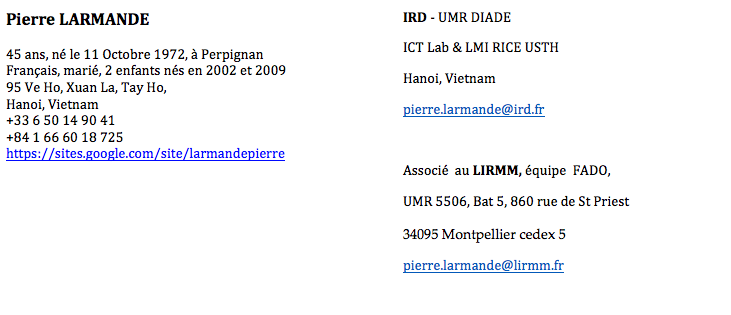
\includegraphics[width=1.0\textwidth]{Figures/CV-img.png}
% \end{center}
%\caption{\label{evol_graph} (Guttler et al. - to appear) An example of evolution graphs ($K$-partite DAG) from a time series of six images.}
% \end{figure}
\begin{center}
\begin{tabular}{cl}
\multicolumn{2}{c}{Pierre LARMANDE} \\
\multicolumn{2}{c}{46 ans, né le 11 Octobre 1972, à Perpignan} \\
\multicolumn{2}{c}{Français, marié, 2 enfants nés en 2002 et 2009} \\
\multicolumn{2}{c}{95 Ve Ho, Xuan La, Tay Ho,} \\
\multicolumn{2}{c}{Hanoi, Vietnam} \\
\multicolumn{2}{c}{+33 6 50 14 90 41} \\
\multicolumn{2}{c}{+84 36 60 18 725} \\
\multicolumn{2}{c}{\url{https://sites.google.com/site/larmandepierre}} \\
\multicolumn{1}{l}{} &  \\
\multicolumn{1}{l}{IRD - UMR DIADE} & Associé au LIRMM \\
\multicolumn{1}{l}{ICT Lab \& LMI RICE USTH} & équipe FADO \\
\multicolumn{1}{l}{Hanoi, Vietnam} & Montpellier, France \\
\multicolumn{1}{l}{pierre.larmande@ird.fr} & pierre.larmande@lirmm.fr
\end{tabular}
\end{center}

\section{Formation}
\begin{description}
    \item[Licence de Biochimie - Maîtrise de Biochimie Université Montpellier 2] : \\ Obtenues en 1995 -1996
    \item[D.E.S.S. Informatique Appliquées aux Organisations Université Montpellier 2] : \\ Obtenu le 2 septembre 2000 à Montpellier, mention assez bien

    \item[Doctorat de 3me cycle Université Montpellier 2] : \\ Soutenu le 20 décembre 2007 à Montpellier, mention très honorable
    \item[]\hspace{0.5cm} \textit{Sujet} :  Mutaliser et partager, un défi pour la génomique fonctionnelle végétale 
    \item[]\hspace{0.5cm}  \textit{Président} : Corinne Cauvet, Professeur d'Université Marseille Nord
    \item[]\hspace{0.5cm}  \textit{Rapporteurs} : Anne Doucet, Directeur de Recherche CNRS (Lyon) et \\
                Christine Froidevaux, Professeur Université Orsay (Paris)
    \item[]\hspace{0.5cm}  \textit{Co-encadants}: Isabelle Mougenot, Maître de conférence Université Montpellier 2 et \\
		Manuel Ruiz, Chercheur Cirad (Montpellier)
    \item[]\hspace{0.5cm} \textit{Directeurs} : Thérèse Libourel, Professeur Université Montpellier 2
   
    

	 	
\end{description} 
%\includepdf[pages={1-7}]{Larmande_manuscript.pdf}
\section{Expérience professionnelle}
\begin{itemize}
\item[Février 2001 – Juillet 2002 ]  \textbf{Bioinformaticien}, CIRAD, UMR PIA, Montpellier \\
Financement : projet Génoplante / CDD CIRAD	
\item[Aout 2002 – Novembre 2005]  \textbf{Bioinformaticien, Ingénieur} CIRAD, UMR PIA, Montpellier \\
Financement : CDD Ingénieur d’Etude CNRS 
\item[Décembre 2005 - Septembre 2010]  \textbf{Bioinformaticien, IE2}, CNRS, Centre d’Ecologie Fonctionnelle Evolutive mis à disposition au CIRAD UMR DAP \\
Financement : Ingénieur d’Etude permanent CNRS, 
\item[Octobre 2010 - Aout 2016]  \textbf{Bioinformaticien, IE2}, IRD, UMR DIADE équipe RICE (Rice, Interspecies Comparison \& Evolution)\\
Financement : Ingénieur d’Etude (IE2) permanent IRD
\item[Septembre 2016 - Octobre 2018]  \textbf{Bioinformaticien, IE2}, IRD, UMR DIADE équipe RICE (Rice, Interspecies Comparison \& Evolution) – scientifique associé équipe FADO (LIRMM)\\
En affectation au Vietnam (Hanoi). Co-Directeur du laboratoire d’informatique ICTLab de l’USTH.
\item[Novembre 2018 - En cours]  \textbf{Chercheur, CRCN}, IRD, UMR DIADE équipe RICE (Rice, Interspecies Comparison \& Evolution) – scientifique associé équipe FADO (LIRMM)\\
En affectation au Vietnam (Hanoi). Co-Directeur du laboratoire d’informatique ICTLab de l’USTH.

\end{itemize}

\vspace{1cm}
\textbf{Domaines de recherche} : 	Bio-ontologies, intégration des données et connaissances, Web Sémantique, Génomique, Agronomie
